\documentclass[]{article}
\usepackage{lmodern}
\usepackage{truncate}
\usepackage{caption}
\usepackage{tocloft}
\usepackage{amssymb,amsmath}
\usepackage{ifxetex,ifluatex}
\usepackage{fixltx2e} % provides \textsubscript
\usepackage{longtable}
\usepackage{graphicx}
\usepackage[table]{xcolor}


\setlength{\parindent}{0pt}
\setlength{\parskip}{6pt plus 2pt minus 1pt}
\setlength{\emergencystretch}{3em}  % prevent overfull lines

\usepackage[breaklinks=true]{hyperref}
\hypersetup{colorlinks,%
citecolor=blue,%
filecolor=blue,%
linkcolor=blue,%
urlcolor=blue}
\usepackage{url}
\usepackage{caption}
\usepackage{cleveref}
\usepackage{booktabs}
\usepackage{fancyvrb}
\usepackage[english]{babel}
\usepackage{geometry}
\geometry{verbose,letterpaper,tmargin=1in,bmargin=1in,lmargin=1in,rmargin=1in}

\usepackage{titlesec, blindtext, color}
\definecolor{gray75}{gray}{0.75}
\newcommand{\hsp}{\hspace{20pt}}

% Headers and page numbering
\usepackage{fancyhdr}
\pagestyle{fancy}
\lhead{  \nouppercase  \leftmark}
\rhead{\thepage}
\cfoot{}

% titles
\usepackage{titling}
\pretitle{\Large}
\posttitle{ \\}
\preauthor{\large}
\postauthor{}
\predate{\large}
\postdate{}

% figure float
\usepackage{float}
\floatplacement{figure}{h}
\usepackage{morefloats}

% section titles
\usepackage{sectsty}
\setcounter{secnumdepth}{1}
\usepackage[normalem]{ulem}
\sectionfont{\rmfamily\Large}
\subsectionfont{\rmfamily\upshape\large}
\subsubsectionfont{\rmfamily\normalsize}

% natbib
\usepackage[square, numbers]{natbib}
\bibliographystyle{unsrtnat}


\hyphenpenalty 1000
% line spacing
\usepackage{setspace}
\linespread{1.2}
\raggedbottom


% define title
\title{Committee Report 2020}
\author{M.D. Catchen}
\date{}

\begin{document}

\maketitle

\vspace{3em}
\subsubsection*{Abstract}

As Anthropogenic activity rapidly reshapes our planet, forecasting the future of Earth's ecosystems and the services they provide humanity poses an immense but necessary challenge. The infrastructure for the collection and assimilation of the data required to model ecosystems at global scales is still in its infancy. Further, robust prediction has long evaded ecological processes due to their inherently complex, stochastic, and emergent nature.
Many disciplines that deal with similarly complex phenomena have benefited from using simulation models as tools for both inference and prediction, but in this realm, ecology has been a slow adopter. We contest is much to be gained in biodiversity science from the further adoption of these methods as regular.
Here, we argue for the potential of simulation models in ecological forecasting, and propose a dissertation which explores the ``forecastability" of ecological systems, presents a framework and software for forecasting the dynamics ecological communities at the scale of metacommunity dynamics, and examines the road toward forecasting the ``rewiring'' of ecological communities in the Anthropocene.

    
\clearpage
\section{Introduction}

Humans have long sought to forecast natural phenomena. For ages, people have attempted to predict the weather, the movement of celestial bodies,  eclipses, natural disasters, and plagues---largely unsuccessfully aside from the occasional false positive. The principles used to develop predictions about the world have varied widely, but of the methods attempted thus far, quantitative models have proven ``unreasonably effective" in predicting nature's behavior \cite{unreasonable_effectiveness}. Yet, it seems that some systems are more inherently more ``forecastable" than others.
Edmund Halley's hand computations enabled him to predict the return of his now eponymous comet 53 years in advance, but predicting the weather further than two weeks in the future is generally considered impossible (with contemporary computing power) \cite{numerical_weather}. 
In ecology, we have faced significant difficulty accurately predicting the outcomes of ecological processes---yet as anthropogenic activity drives rapid changes in our planet, forecasting ecological processes remains a vital challenge to help mitigate biodiversity loss and its impacts on humanity \cite{dietze_forecasting_2019, pereira2010scenarios}.

Why has forecasting ecological systems proven so difficult? 
Biological systems (and complex systems more generally) often evade effective prediction because internal heterogeneity propagates from smaller toward larger scales \citep{levins_dialectical_1987,levin_problem_1992}. The process of developing a quantitative model (for forecasting or other purposes) has long been one of \textit{reductionism}: a system is divided into parts, and those parts subdivided into parts further until no more subdivision is possible, at which point we study the atomic parts the our system in order to build our understanding from the ``bottom-up". However, the properties of complex systems are emergent, and
Levins and Lewontin \cite{levins_dialectical_1987} argue that reductionism fails in ecology because there is not a single ``true" scale from which higher level phenomena arise---instead there is a dialectical nature between part and whole: neither determines the other, but instead the behavior of complex systems must be understood as a synthesis of ``bottom-up'' and ``top-down'' effects. They write 

\begin{quote}
Idealism and reductionism in ecology share a common faults: they see ``true causes" as arising at one level only, with other levels having epistemological but not ontological validity...A space capsule could not land on the moon without Newtonian abstractions, nor could it land with them alone. The problem for science
is to understand the proper domain of explanation of each abstraction
rather than become its prisoner. \citep{levin_problem_1992}
\end{quote}

We argue that simulation models can aid us in ecological inference and forecasting because they allow us to explore the ``proper domain of explanation of each abstraction" more explicitly than the conventional statistical models often applied in ecological research, while providing more information about process than machine learning models. Using dynamics simulations, we contest, we can directly compare process-based models which incorporate heterogeneity and stochasticity across scales in order to determine which best explain empirical data. The ongoing development of likelihood-free methods for inference to confront simulation models with data has seen interest across fields \cite{alsing_massive_2018, didelot_likelihood-free_2011, drovandi_likelihood-free_2011,orbanz_bayesian_2015}. These tools have been applied for forecasting and inference in other complex systems---numerical weather prediction has vastly improved its forecasting ability with the advent of the computing power to run large numbers of dynamical simulations (Appendix Figure \ref{fig:num_weather},  \cite{numerical_weather}). We contest biodiversity science has much to gain in adopting these methods as regular. There are certainly challenges in this domain---how do we find a bridge between complex simulation models and data? How do we validate that these simulation models make  correct predictions?
How much data would we need to accurately forecast an ecological system? On what spatial and temporal scales are out forecasts valid? 
These are the questions which this dissertation will aim to answer.


\clearpage
\section{Proposed Dissertation Structure}
Out of the vast amount of ecological information we could attempt to forecast, we focus on two distinct but related problems related to dynamics and structure of Earth's ecological communities. We focus on two scales of interest---first: forecasting metacommunity dynamics (the occupancy/abundance of species across space) on spatiotemporal scales where the metaweb is fixed, and second: forecasting the composition of the metaweb on spatiotemporal scales where changes in range-limits drive the ``rewiring'' of ecological communities. We propose the following four chapters:
First, a review of the relevant literature surrounding the core topics of the dissertation: models, spatial ecology, ecological networks, and forecasting. Second, a software toolkit, MetacommunityDynamics.jl (MCD.jl) for analysis and forecasting of metacommunity dynamics. Third, an investigation of the forecasting horizon of metacommunities, using MCD.jl. And finally, a framework for forecasting the future rewiring of ecological networks under climate and land-use change.

\subsection{Chapter One --- Introduction and Review}

This chapter aims to introduce the subject of the dissertation and summarize the relevant work from the literature that will be built upon in the following chapters. Here, I'll briefly summarize the topics covered, in part to determine where the gaps in my reading are. The topics covered roughly fall into the categories

\begin{enumerate}
    \item Models and Inference in Ecology \\ \hfill \\
        A look at the epistemological background of modeling and probability  \cite{jaynes_probability,crutchfield_semantics, pearl_causality}, the different purposes the models serve (inference, prediction, forecasting), an overview of the benefits and limitations of the modeling strategies historically and currently used in ecology \cite{whitlock2009analysis, mcelreath2020statistical}.
    \item Spatial Ecology \\ \hfill \\
        An overview of the history of spatial ecology, beginning with the Theory of Island Biogeography \cite{macarthur_theory_1969}, metapopulation theory \cite{levins_demographic_1969}, the theory of sources and sinks \cite{pulliam1988sources}, spatially-explicit metapopulation theory \cite{hanski_practical_1994, ovaskainen_metapopulation_2002} and occupancy modeling \cite{ howell2018increasing}, landscape genetics and resistance surfaces \cite{manel_landscape_2003, mcrae_isolation_2006, mcrae_using_2008, mcrae_isolation_2006, mcrae_using_2008}, connectivity \cite{taylor_connectivity_1993,kool_population_2013}, spatial graphs \cite{chubaty_r_2020,dale_graphs_2010,minor_graph-theory_2008, urban_landscape_2001},  species distribution modeling \cite{elith2009species, kissling2018building, pollock2014understanding}.
    \item Community Ecology
        \\ \hfill \\
        Classic community ecology \cite{hutchinson_homage_1959, macarthur_competition_1964, macarthur_patterns_1965, macarthur_limiting_1967,macarthur_species_1970,macarthur_theory_1969}, 
        May's original work on diversity and stability \cite{may_will_1972, may_stability_2001},
        allometry and thermodynamic models \cite{cohen_food_1977, yodzis_body_1992, brose_allometric_2006, stouffer_robust_2006, otto_allometric_2007, gravel_trophic_2011, delmas_simulations_2017}, metacommunity theory \cite{leibold_metacommunity_2004} and process-based models of metacommunity structure \cite{vellend_conceptual_2010}, generative models of food-webs \cite{cohen_food_1977,williams_simple_2000,allesina_general_2008,thompson_process-based_2020}, network theory  \cite{ clauset_finding_2004,newman_modularity_2006, olesen_modularity_2007,neutel_reconciling_2007,larremore_bipartite_sbm} and its application to ecology \cite{bascompte_nested_2003,bascompte_asymmetric_2006,allesina_stability_2012,allesina_predicting_2015, delmas_food_2020, Delmas2018, delmas_simulations_2017}.
    \item Forecasting  \\ \hfill \\
        A review of the general forecasting problem (Figure \ref{fig:inference_prediction_forecasting}) and its relation to inverse and forward problems \cite{stouffer_all_2019},  forecasting in nonlinear systems
        \cite{crutchfield_semantics}, ensemble modeling \cite{parker2013ensemble}, ecological forecasting  and adaptive management \cite{dietze_ecological_2017, dietze_iterative_2018}.
        
        \begin{figure}[H]
    \centering
    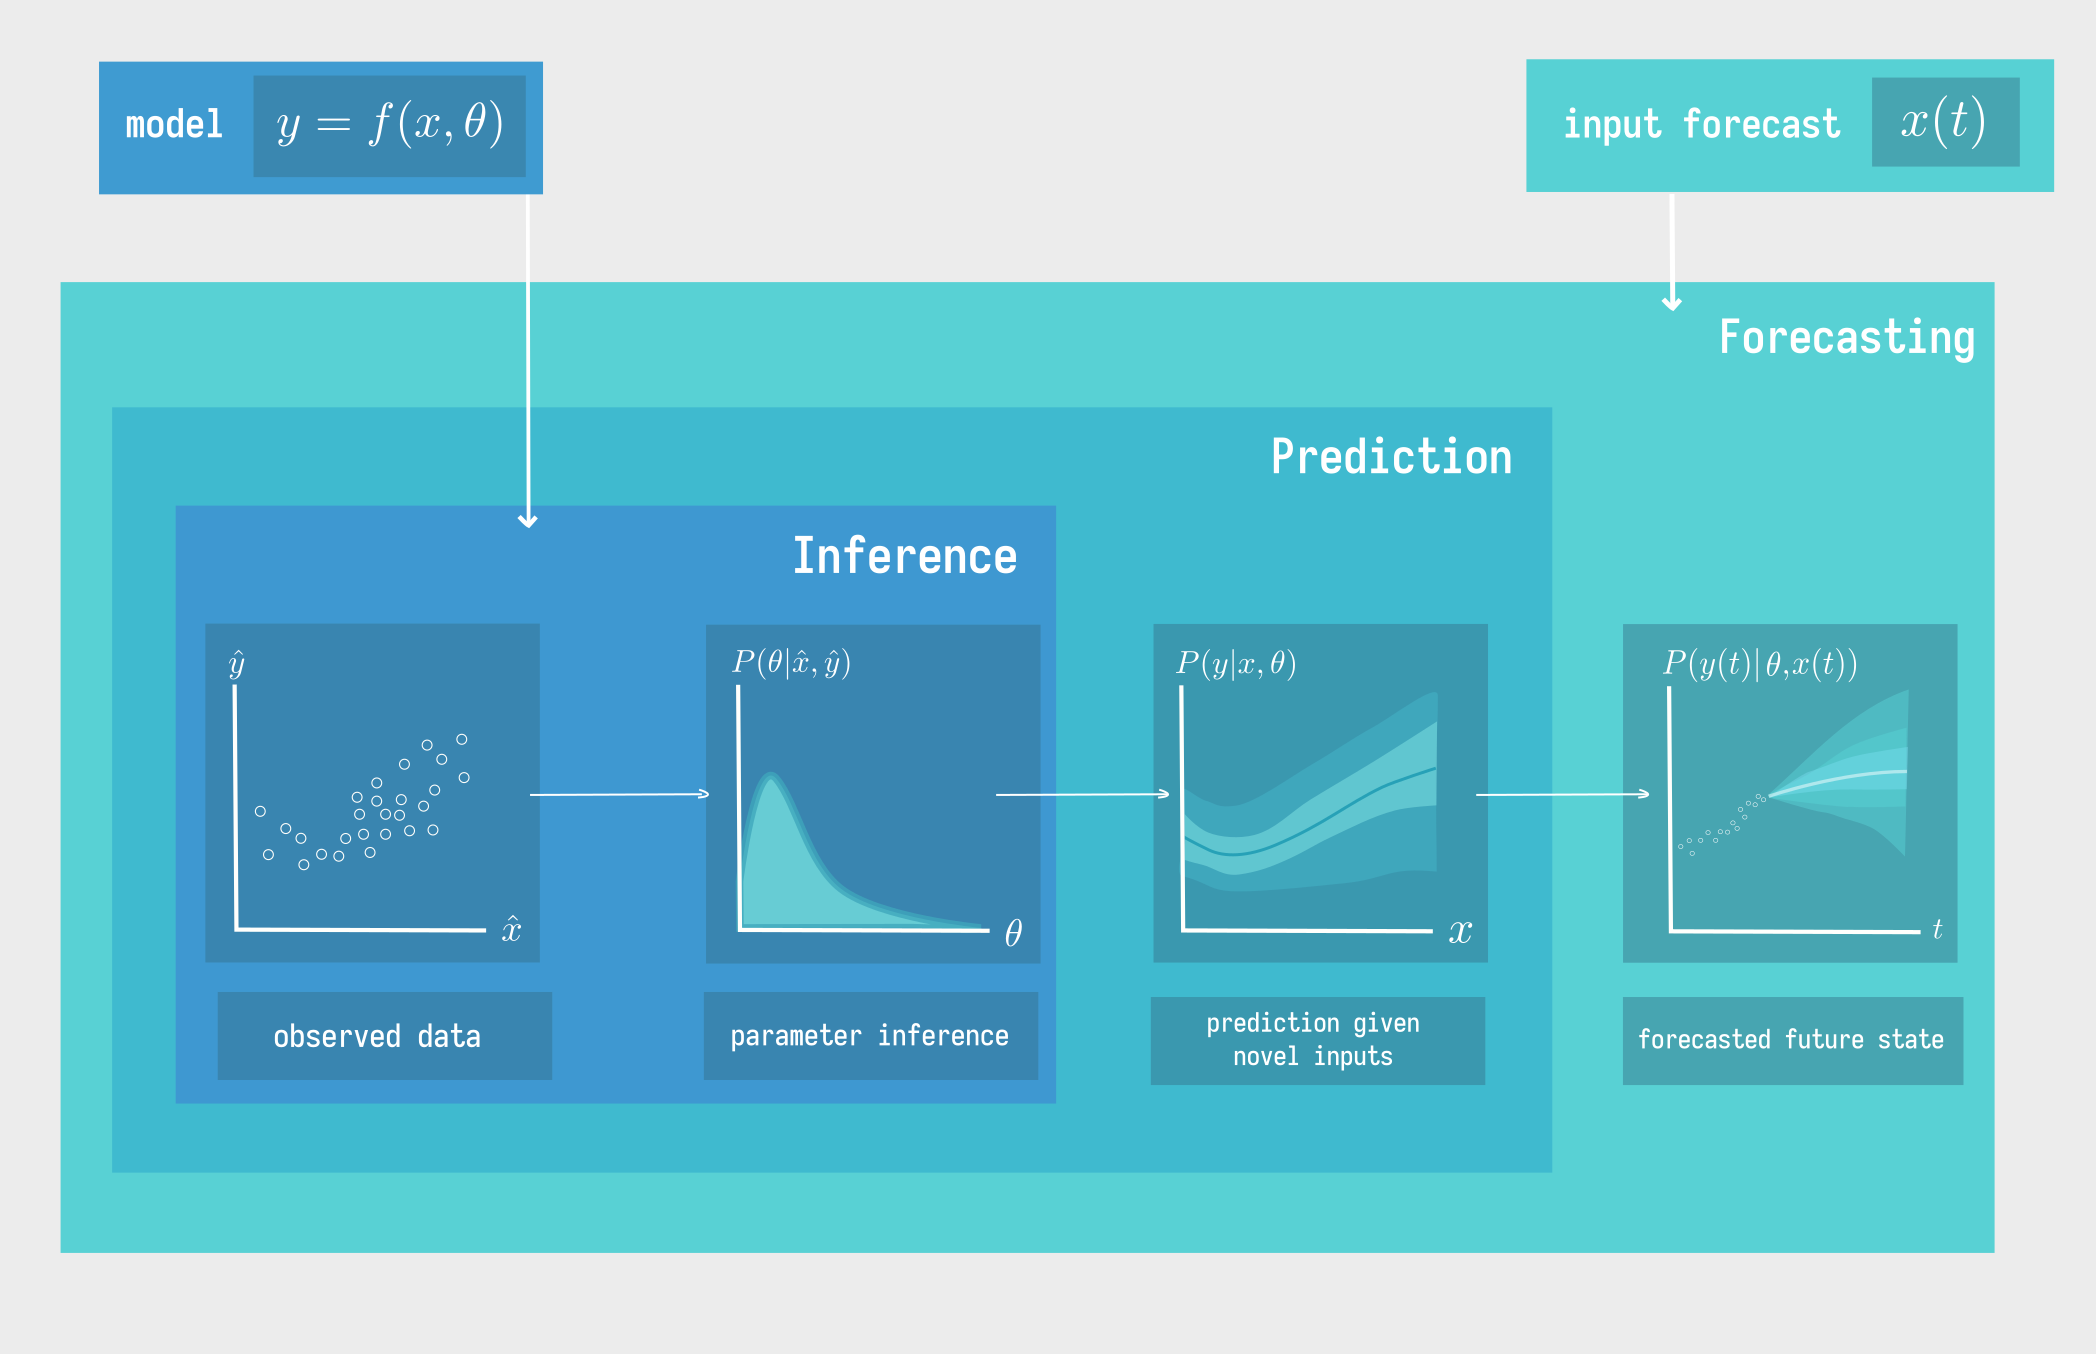
\includegraphics[width=17cm]{figs/inf_prediction_forecasting.png}
    \caption{The Forecasting Problem. Forecasting inevitably requires assuming a model $f$, which maps inputs $x$ and parameters $\theta$ to outputs, $y$. The first step of forecasting is inference, we where take observed measurements of both outputs $\hat{y}$ and inputs $\hat{x}$, and estimate the $\theta$ based on this information (often called the inverse problem \cite{stouffer_all_2019}). We then use our estimate of $\theta$ to make predictions about the values of $y$ given novel inputs, $x$. Finally, given a forecast of the inputs, $x(t)$, we can use the model to forecast the output state, $y(t)$. }
    \label{fig:inference_prediction_forecasting}
\end{figure}

\end{enumerate}


\subsection{Chapter Two --- MetacommunityDynamics.jl: A software toolkit for analysis and forecasting of metacommunity dynamics }

This chapter presents a software toolkit, MetacommunityDynamics.jl, which includes several generative models of metacommunity dynamics and methods to fit these models to data, including an example of applying it to LEAP data \cite{Bell2019}. The resulting paper from this chapter is targeted at Methods in Ecology and Evolution.
The goal of this software package is to provide the entire pathway of tools required to forecast the dynamics of abundance/occupancy in a metacommunity with a given metaweb, and further, it should interface with the wide variety of existing tools in Julia for the analysis of ecological networks, spatial ecology, and so on. 

The software package can be divided into two components---one which is a generative model of metacommunity dynamics, and the second which is a set tools for fitting this generative model to data. Together,  these components we have the required tools necessary to  forecast metacommunity dynamics.

\subsubsection{Generative Model Component}

The generative model outputs trajectories of metacommunity dynamics under a given parameters $\theta$, represented as a tensor $B$ (Figure \ref{fig:software}).

The software should be capable of interfacing with an empirical metaweb, landscape, trait distribution, and so on (see Figure \ref{fig:software}), while also providing generative models of each of these components such that the software can also be used as a "virtual laboratory" for exploring the properties of metacommunities without empirical information. The generative model itself consists of two parts, a model of the 
spatial domain where the dynamics unfold, represented as a spatial graph (Appendix Figure \ref{fig:spatial_models}), and a model of community dynamics at the `local' spatial scale---as part of MCD.jl, I plan to implement several models of community dynamics \cite{thompson_process-based_2020, elkof_bayesian_2013} models, as well as utilizing existing software \cite{delmas_simulations_2017}.

\begin{figure}[h]
    \centering
    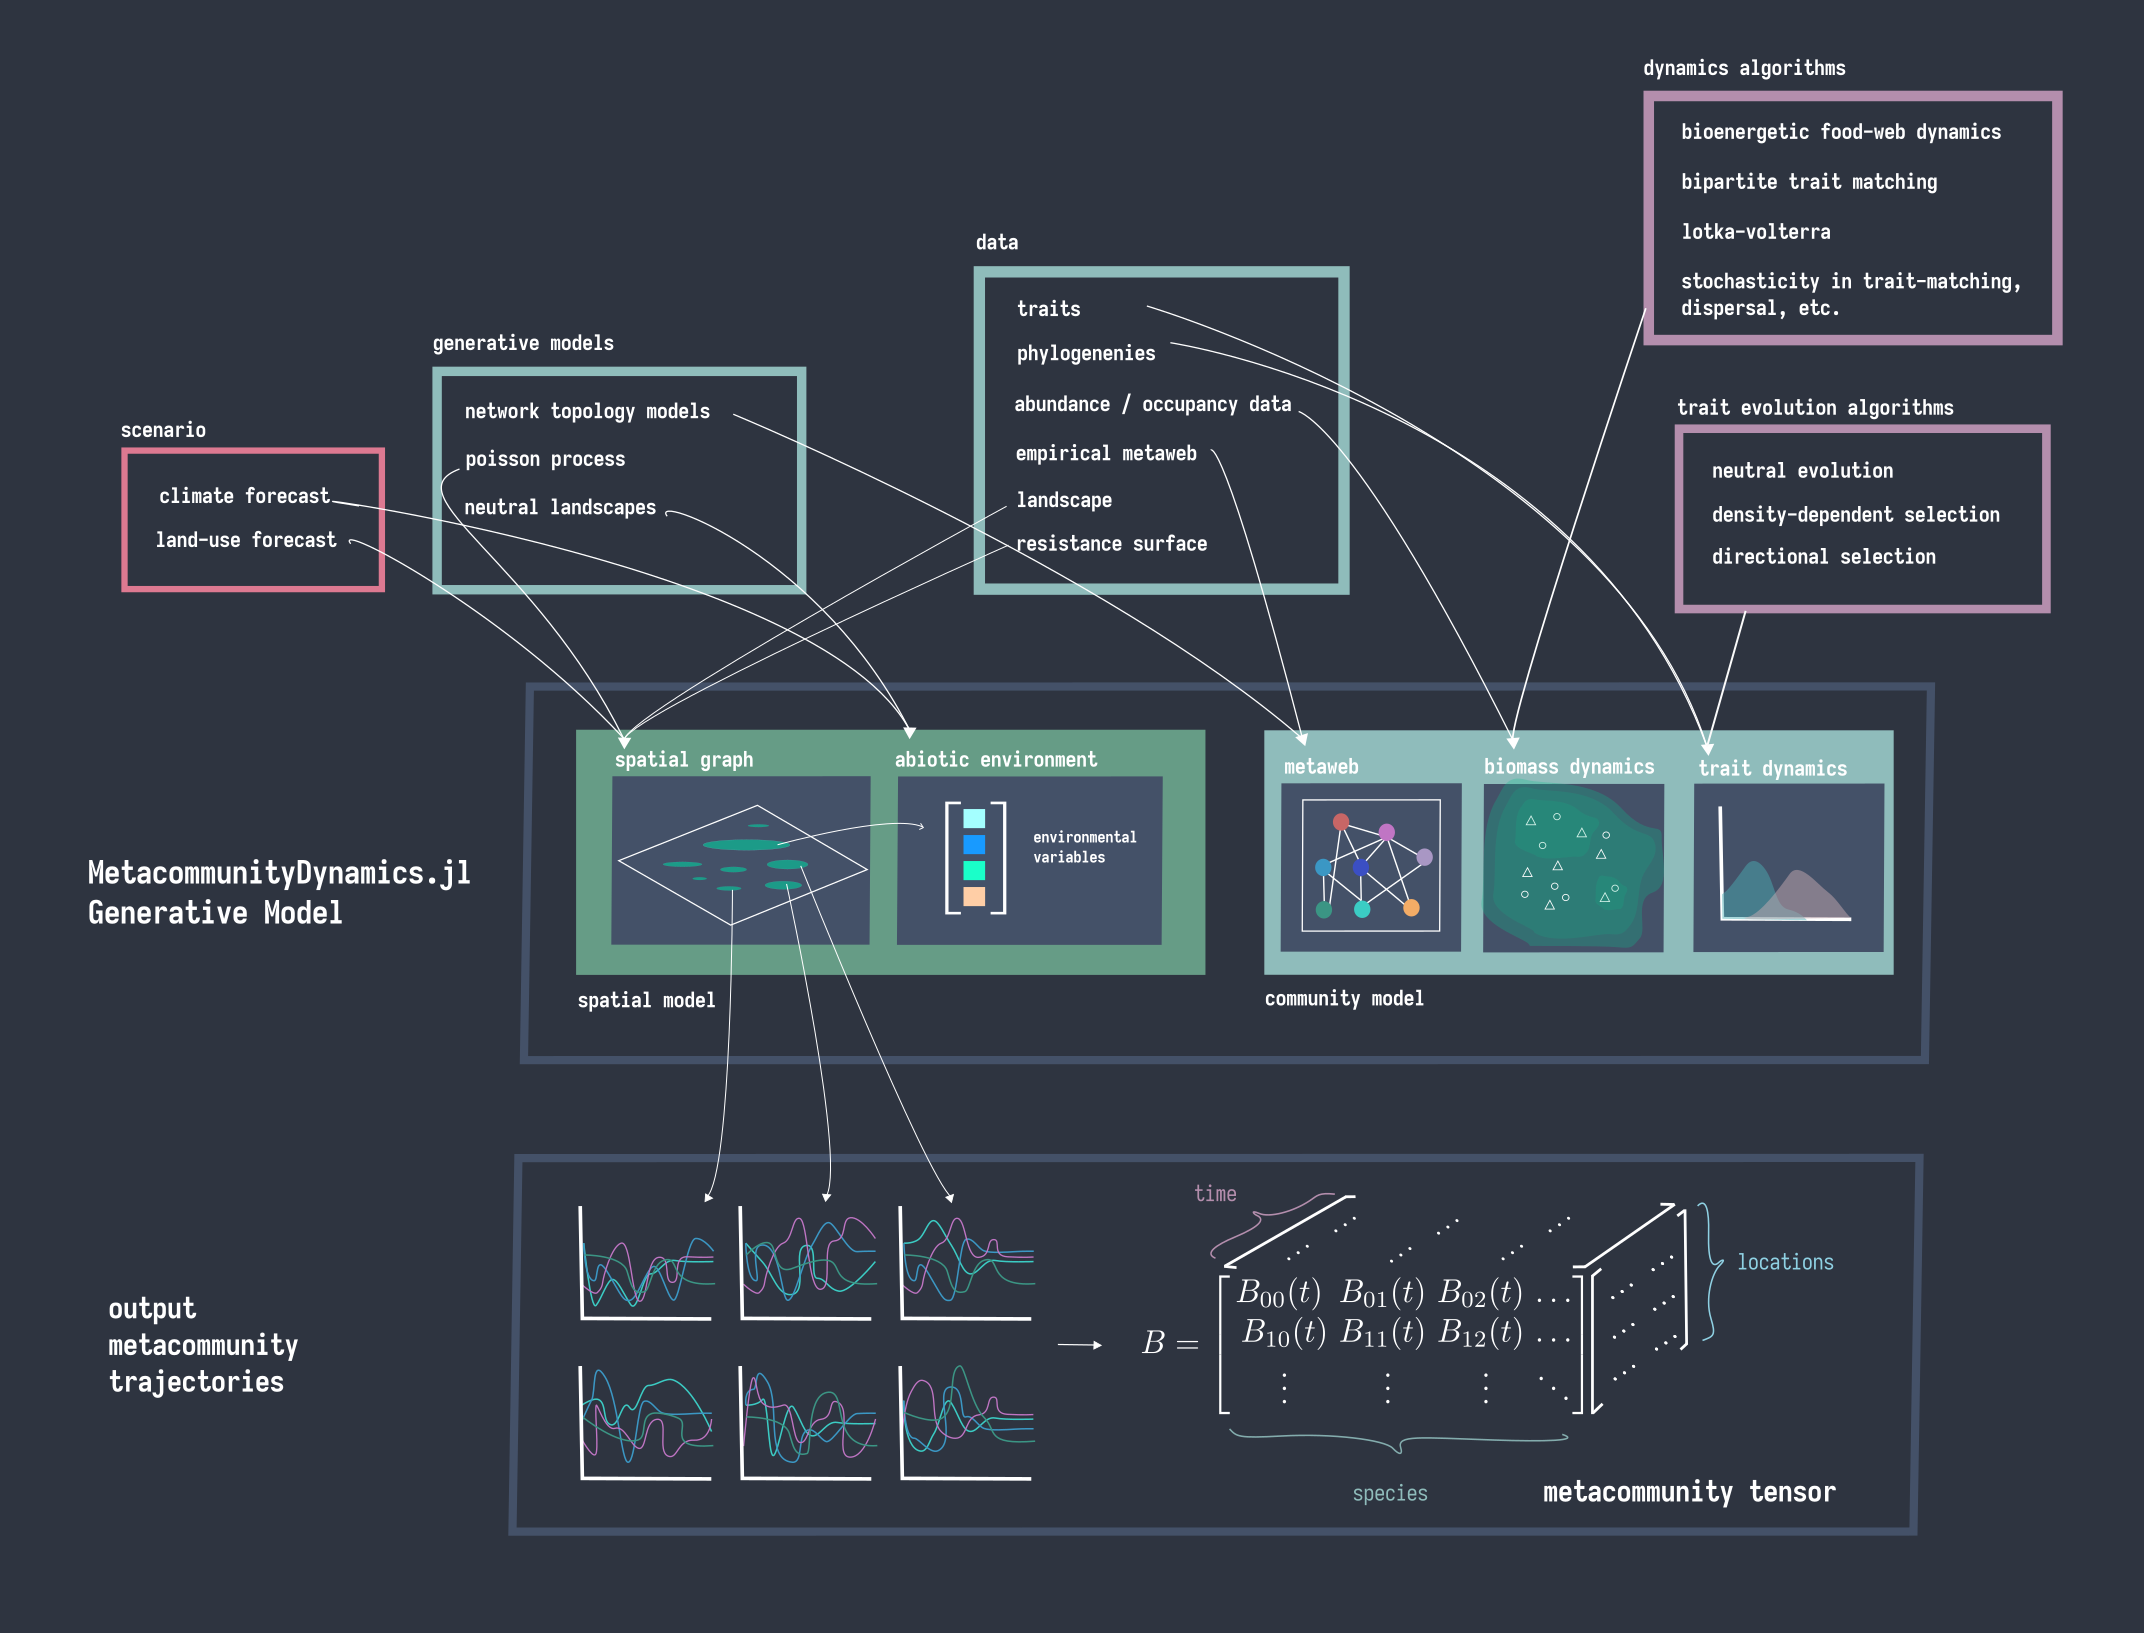
\includegraphics[width=17cm]{figs/software.png}
    \caption{The generative model component of MetacommunityDynamics.jl (MCD.jl). The component produces trajectories of metacommunity dynamics (either in occupancy or abundance space) as tensors, using either empirical metaweb/landscape/trait data, or generated features.} 
    \label{fig:software}
\end{figure}


\subsubsection{Inference Component}

The inference component is concerned taking empirical metacommunity occupancy/abundance data, represented as a tensor $\hat{B}$, and inferring the parameters under a given model of dynamics (the \textit{Inference} box of  Figure \ref{fig:inference_prediction_forecasting}). In order to do this, we consider implementing a few methods of likelihood-free inference, which can estimate the parameters $\theta$ responsible for generating tensors $B$ that are statistically similar to $\hat{B}$ under a given generative model of dynamics. The methods I'm considering implementing are 1) Approximate Bayesian Computation \cite{beaumont_approximate_2019}, 2) Generative Anatagonistic Networks \cite{radford2015unsupervised}, and 3) Optimal Transport Theory \cite{cuturi_opt}. These each provide a framework for fitting generative models to data, and some general software packages for implementing these methods already exist in Julia.   

Further, the component responsible for inference should also provide tools for model validation. In this case, we can think about validation in two ways---one is to give the model data one timestep at a time, and validate its predictive accuracy at each round of new data. The second is to train the model on all temporal data and crossvalidate its prediction across different locations. In addition, this component should be able to apply information criteria in order to predict which dynamics model performs best on the dataset. 



\subsection{Chapter Three --- The Forecasting Horizon of Metacommunity Dynamics}

Forecasting inherently operates on a given timescale.
On some timescales, forecasting ecological systems is trivial \cite{crutchfield_semantics}---the species composition of a given ecosystem now and an hour from now is likely to be same. On the other hand, its not feasible to attempt to predict the composition of ecological communities hundreds of years in the future. The aim of this chapter is to investigate where in-between these time scales we can make useful forecasts of metacommunity dynamics. We will do this by using the generative model component of MPD.jl to generate dynamics, and then use the inference component of MPD.jl to forecast the dynamics trajectory as if we know nothing the source generating it. 
Further, we hope to explore the resolution limit of forecasting (how accurately we could predict abundance given perfect information), how much data is required to make accurate forecasts, and how much measurement error is acceptable until the sytsem becomes unforecastable.

As a case-study of this, here we investigate the forecasting horizon of a double pendulum---a classic example of chaotic dynamics. In Figure \ref{fig:forecasting_horizon}, we see the forecasting horizon of a double-pendulum at various levels of measurement error, and that the amount of measurement error affects the timescales on which we can make valid forecasts. 

\begin{figure}[h]
    \centering
    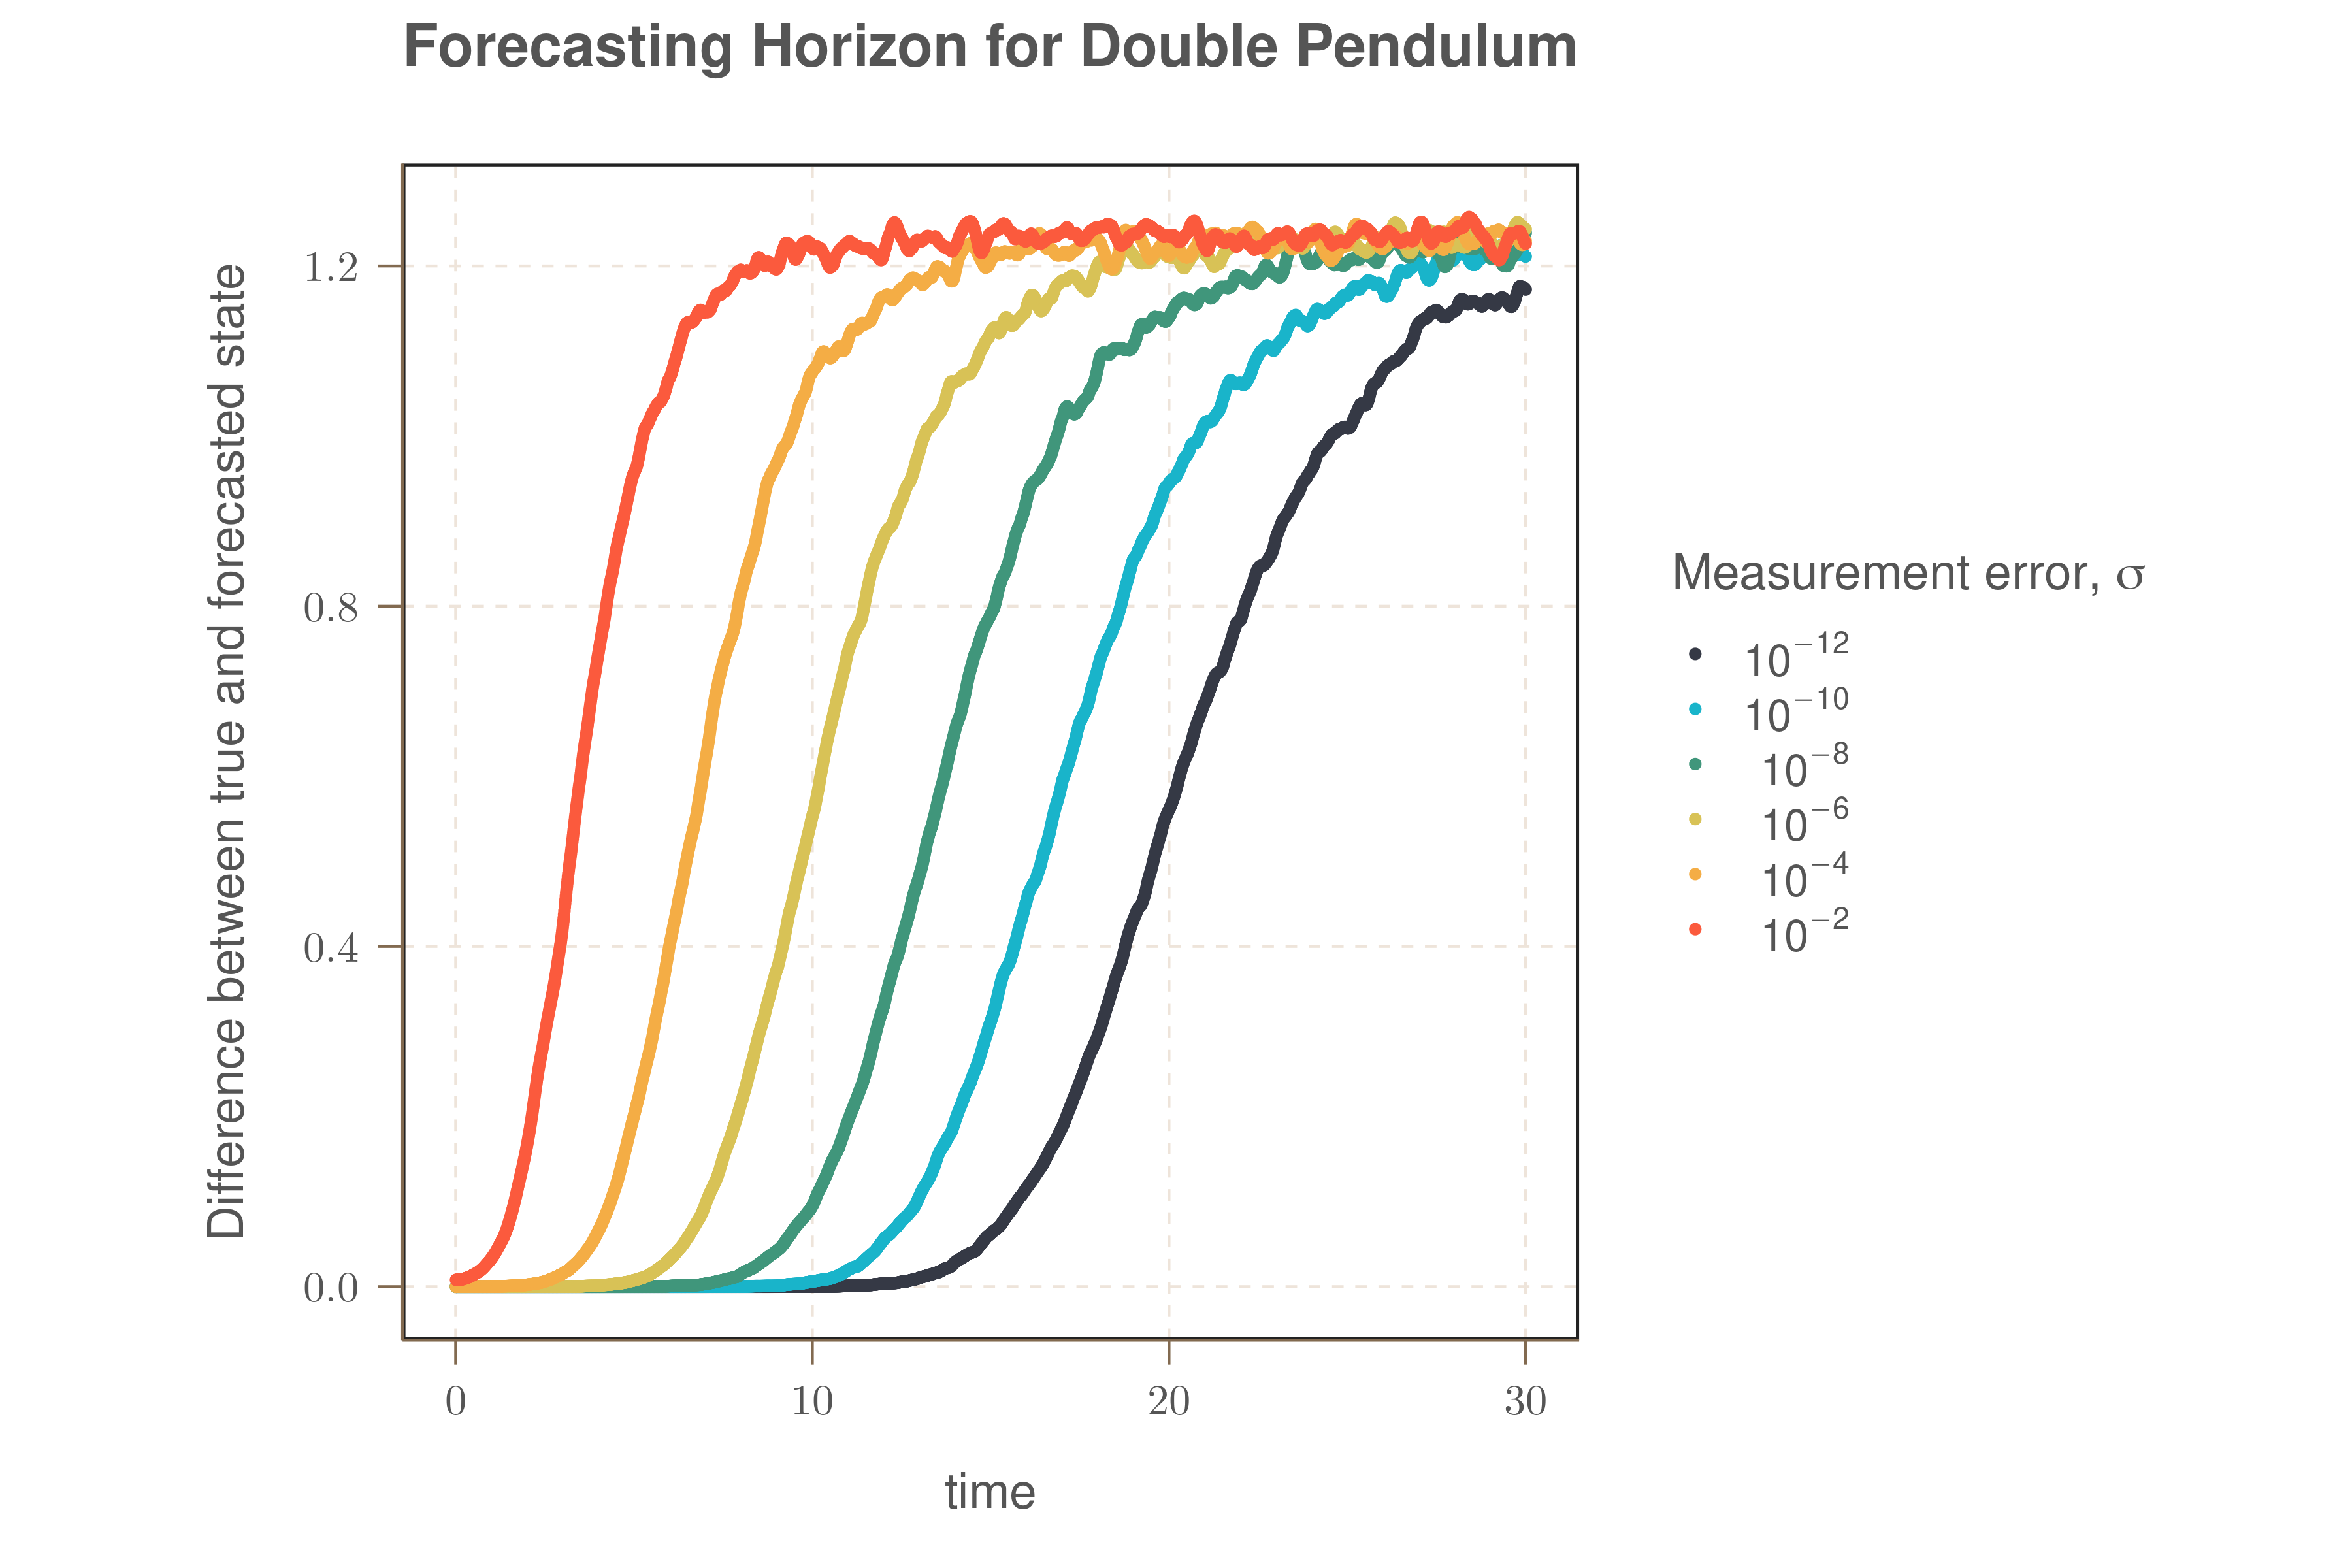
\includegraphics[width=17cm]{figs/forecasting_horizon.png}
    \caption{The error in a forecast of a double pendulum's position at various levels of inherent measurement error, $\sigma$. For 2000 replicates, a double pendulum was simulated with true initial condition $\{ \theta_1, \theta_2 \}$ and measured initial condition $\{\theta_A, \theta_B \}$, where measurement error is simulated by setting $\theta_A = \theta_1 + \epsilon_1$ and $\theta_B = \theta_2 + \epsilon_2$, with $\epsilon_1, \epsilon_2 \sim N(0, \sigma)$ at the start of each replicate. Then, the trajectories of both the true pendulum with state $(\theta_1, \theta_2)$ and measured pendulum $(\theta_A, \theta_B)$ are integrated forward. The distance between the position of the true and forecasted outermost pendulum (averaged across replicates) is shown on the plot as a function of time, with different $\sigma$ in different colors. For all simulations, both pendulums have length $1$.}
    \label{fig:forecasting_horizon}
\end{figure}

The goal of this chapter is to take this idea and apply it to metacommunity dynamics. In addition to measurement error, we plan to explore the how the forecasting horizon changes as a function of how much data is available, how well we understand the ``true" dynamics governing the system. 

\subsection{Chapter Four --- The path toward forecasting the future of Earth's ecological communities}

This chapter outlines the path toward  forecasting on spatiotemporal scales where changes in  range-limits cause the ``rewiring'' of ecological communities. The first step toward this is prediction of networks across space---this first part of this chapter will overlap with the spatial network prediction paper we are collectively working on, which develops a roadmap toward prediction of networks across space (Figure \ref{fig:network_prediction}). 
After we have a framework for spatial prediction, we will then what data would be required to forecast the rewiring of metawebs into the future. 


\begin{figure}[h]
    \centering
    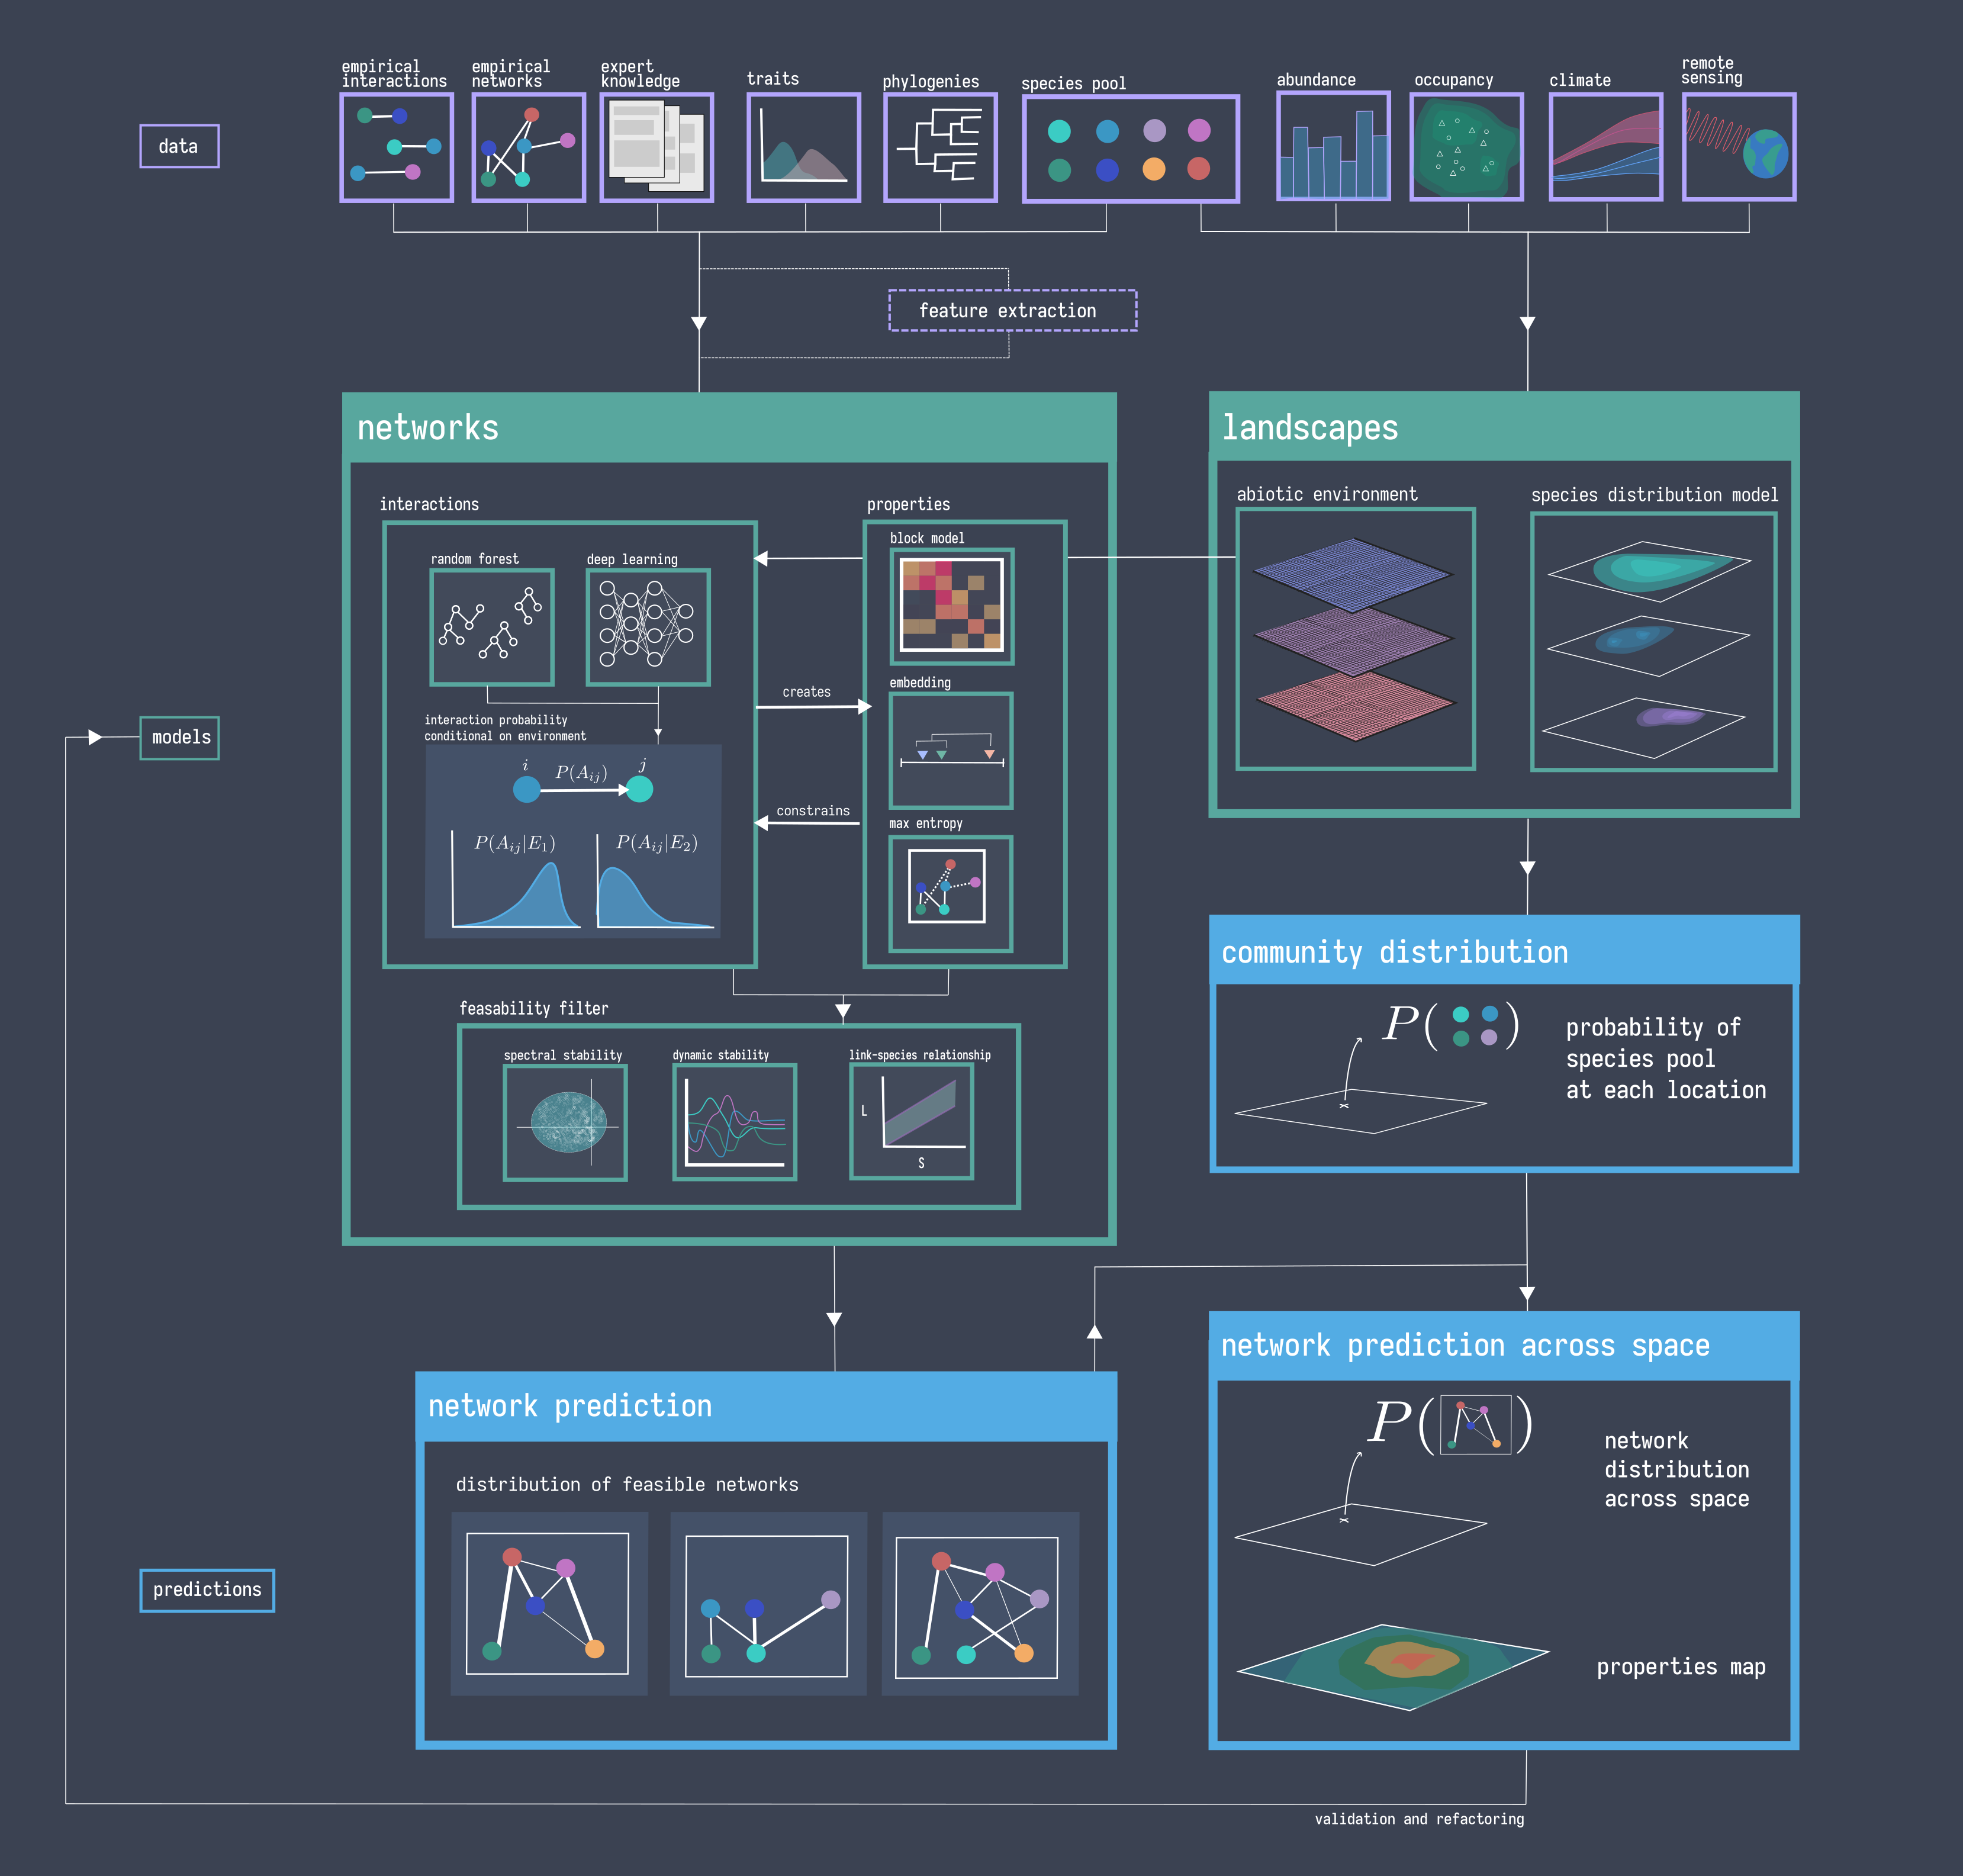
\includegraphics[width=17cm]{figs/combined_spatial_network_prediction_v4.png}
    \caption{The flow from data to spatial network predictions (conceptual figure from in-progress spatial network prediction paper)}
    \label{fig:network_prediction}
\end{figure}


\clearpage
\section{Proposed Work}
In the next year, the work I want to get done can be divided roughly into 
\begin{enumerate}
    \item Masters Paper \hfill \\
    The first paper from my masters is almost done, I want to get it submitted by the end of this year.

    \item MetacommunityDynamics.jl (MCD.jl) (Chapter Two, prerequsite for Chapter Three) \hfill \\
    The work in the next year for developing the software package is to look into existing capabilities of existing Julia libraries that already implement functionality I need, draft a design document which more verbosely explains how the software will function, and develop v0.1, which includes the generative model component, and v0.2, which implements the minimal functionality for the inference component.

    \item Network Predictions Paper (part of Chapter Four) \hfill \\ 
    The network predictions paper we are collectively working on will hopefully be submitted early next year.
    
\end{enumerate}

\subsection{Timeline}
\renewcommand{\arraystretch}{1.5}
\begin{table}[H]
\centering
\begin{tabular}{lll} 
\hline
Month                                            & Work                                                                                                                                                                                                                                                                                                                                                                     & Deliverables                                                                   \\ 
\hline
\rowcolor[rgb]{0.949,0.949,0.949} November 2020  & \begin{tabular}[c]{@{}>{\cellcolor[rgb]{0.949,0.949,0.949}}l@{}}\begin{tabular}{@{\labelitemi\hspace{\dimexpr\labelsep+0.5\tabcolsep}}>{\cellcolor[rgb]{0.949,0.949,0.949}}l}\textcolor[rgb]{0.173,0.392,0.643}{Draft Network Prediction Paper}\\\textcolor[rgb]{0,0.502,0.502}{Finish revising masters paper}\end{tabular}\end{tabular}                                &                                                                                \\
December 2020                                    & \begin{tabular}[c]{@{}l@{}}\begin{tabular}{@{\labelitemi\hspace{\dimexpr\labelsep+0.5\tabcolsep}}l}\textcolor[rgb]{0.173,0.392,0.643}{Revise Network Prediction Paper}\\\textcolor[rgb]{0.314,0.227,0.502}{Look into existing Julia libraries}\end{tabular}\end{tabular}                                                                                                 & \textcolor[rgb]{0,0.502,0.502}{Submit masters Paper}                           \\
\rowcolor[rgb]{0.949,0.949,0.949} January 2021   & \begin{tabular}[c]{@{}>{\cellcolor[rgb]{0.949,0.949,0.949}}l@{}}\begin{tabular}{@{\labelitemi\hspace{\dimexpr\labelsep+0.5\tabcolsep}}>{\cellcolor[rgb]{0.949,0.949,0.949}}l}\textcolor[rgb]{0.173,0.392,0.643}{Revise Network Prediction Paper}\\\textcolor[rgb]{0.314,0.227,0.502}{Start MCD.jl design document}\end{tabular}\end{tabular}           &                                                                                \\
February 2021                                    & \begin{tabular}{@{\labelitemi\hspace{\dimexpr\labelsep+0.5\tabcolsep}}l}\textcolor[rgb]{0.314,0.227,0.502}{MCD.jl design document}\end{tabular}                                                                                                                                                                                                                         & \textcolor[rgb]{0.173,0.392,0.643}{Submit Network Prediction Paper}            \\
\rowcolor[rgb]{0.949,0.949,0.949} March 2021     & \begin{tabular}{@{\labelitemi\hspace{\dimexpr\labelsep+0.5\tabcolsep}}>{\cellcolor[rgb]{0.949,0.949,0.949}}l}\textcolor[rgb]{0.314,0.227,0.502}{MCD.jl design document}\end{tabular}                                                                                                                                                                                    & \textcolor[rgb]{0.314,0.227,0.502}{MCD.jl design document v1}                  \\
April 2021                                       & \begin{tabular}[c]{@{}l@{}}\begin{tabular}{@{\labelitemi\hspace{\dimexpr\labelsep+0.5\tabcolsep}}l}\textcolor[rgb]{0.173,0.392,0.643}{Network Prediction Reviews/Resubmit}\\\textcolor[rgb]{0.173,0.392,0.643}{\textcolor[rgb]{0.314,0.227,0.502}{Start Building MCD.jl v0.1}}\end{tabular}\end{tabular}                                                       &                                                                                \\
\rowcolor[rgb]{0.949,0.949,0.949} May 2021       & \begin{tabular}[c]{@{}>{\cellcolor[rgb]{0.949,0.949,0.949}}l@{}}\begin{tabular}{@{\labelitemi\hspace{\dimexpr\labelsep+0.5\tabcolsep}}>{\cellcolor[rgb]{0.949,0.949,0.949}}l}\textcolor[rgb]{0.173,0.392,0.643}{Revise Network Prediction Paper}\\\textcolor[rgb]{0.173,0.392,0.643}{\textcolor[rgb]{0.314,0.227,0.502}{Building MCD.jl v0.1}}\end{tabular}\end{tabular} &                                                                                \\
June 2021                                        & \begin{tabular}{@{\labelitemi\hspace{\dimexpr\labelsep+0.5\tabcolsep}}l}\textcolor[rgb]{0.173,0.392,0.643}{\textcolor[rgb]{0.314,0.227,0.502}{Building MCD.jl v0.1}}\end{tabular}                                                                                                                                                                                        & \textcolor[rgb]{0.173,0.392,0.643}{Resubmit Network Prediction Paper}  \\
\rowcolor[rgb]{0.949,0.949,0.949} July 2021      & \begin{tabular}{@{\labelitemi\hspace{\dimexpr\labelsep+0.5\tabcolsep}}>{\cellcolor[rgb]{0.949,0.949,0.949}}l}\textcolor[rgb]{0.314,0.227,0.502}{Start drafting MCD.jl paper}\end{tabular}                                                                                                                                                                                & \textcolor[rgb]{0.314,0.227,0.502}{MCD.jl v0.1}                                \\
August 2021                                      & \begin{tabular}[c]{@{}l@{}}\begin{tabular}{@{\labelitemi\hspace{\dimexpr\labelsep+0.5\tabcolsep}}l}\textcolor[rgb]{0.314,0.227,0.502}{MCD.jl paper}\\\textcolor[rgb]{0.314,0.227,0.502}{Building MCD.jl v0.2}\end{tabular}\end{tabular}                                                                                                                                  &                                                                                \\
\rowcolor[rgb]{0.949,0.949,0.949} September 2021 & \begin{tabular}[c]{@{}>{\cellcolor[rgb]{0.949,0.949,0.949}}l@{}}\begin{tabular}{@{\labelitemi\hspace{\dimexpr\labelsep+0.5\tabcolsep}}>{\cellcolor[rgb]{0.949,0.949,0.949}}l}\textcolor[rgb]{0.314,0.227,0.502}{Building MCD.jl v0.2}\\\textcolor[rgb]{0.314,0.227,0.502}{MCD.jl paper}\end{tabular}\end{tabular}                                                        &                                                                                \\
October 2021                                     & \begin{tabular}[c]{@{}l@{}}\begin{tabular}{@{\labelitemi\hspace{\dimexpr\labelsep+0.5\tabcolsep}}l}Committee Report 2021\\\textcolor[rgb]{0.314,0.227,0.502}{Begin exploring fitting MPD.jl to LEAP data}\end{tabular}\end{tabular}                                                                                                                                      & \textcolor[rgb]{0.314,0.227,0.502}{MPD.jl v0.2}                               
\end{tabular}
\end{table}

{
\linespread{0.9}
\footnotesize
\bibliography{refs}
}

\clearpage
\section{Appendix}

\begin{figure}[h]
    \centering
    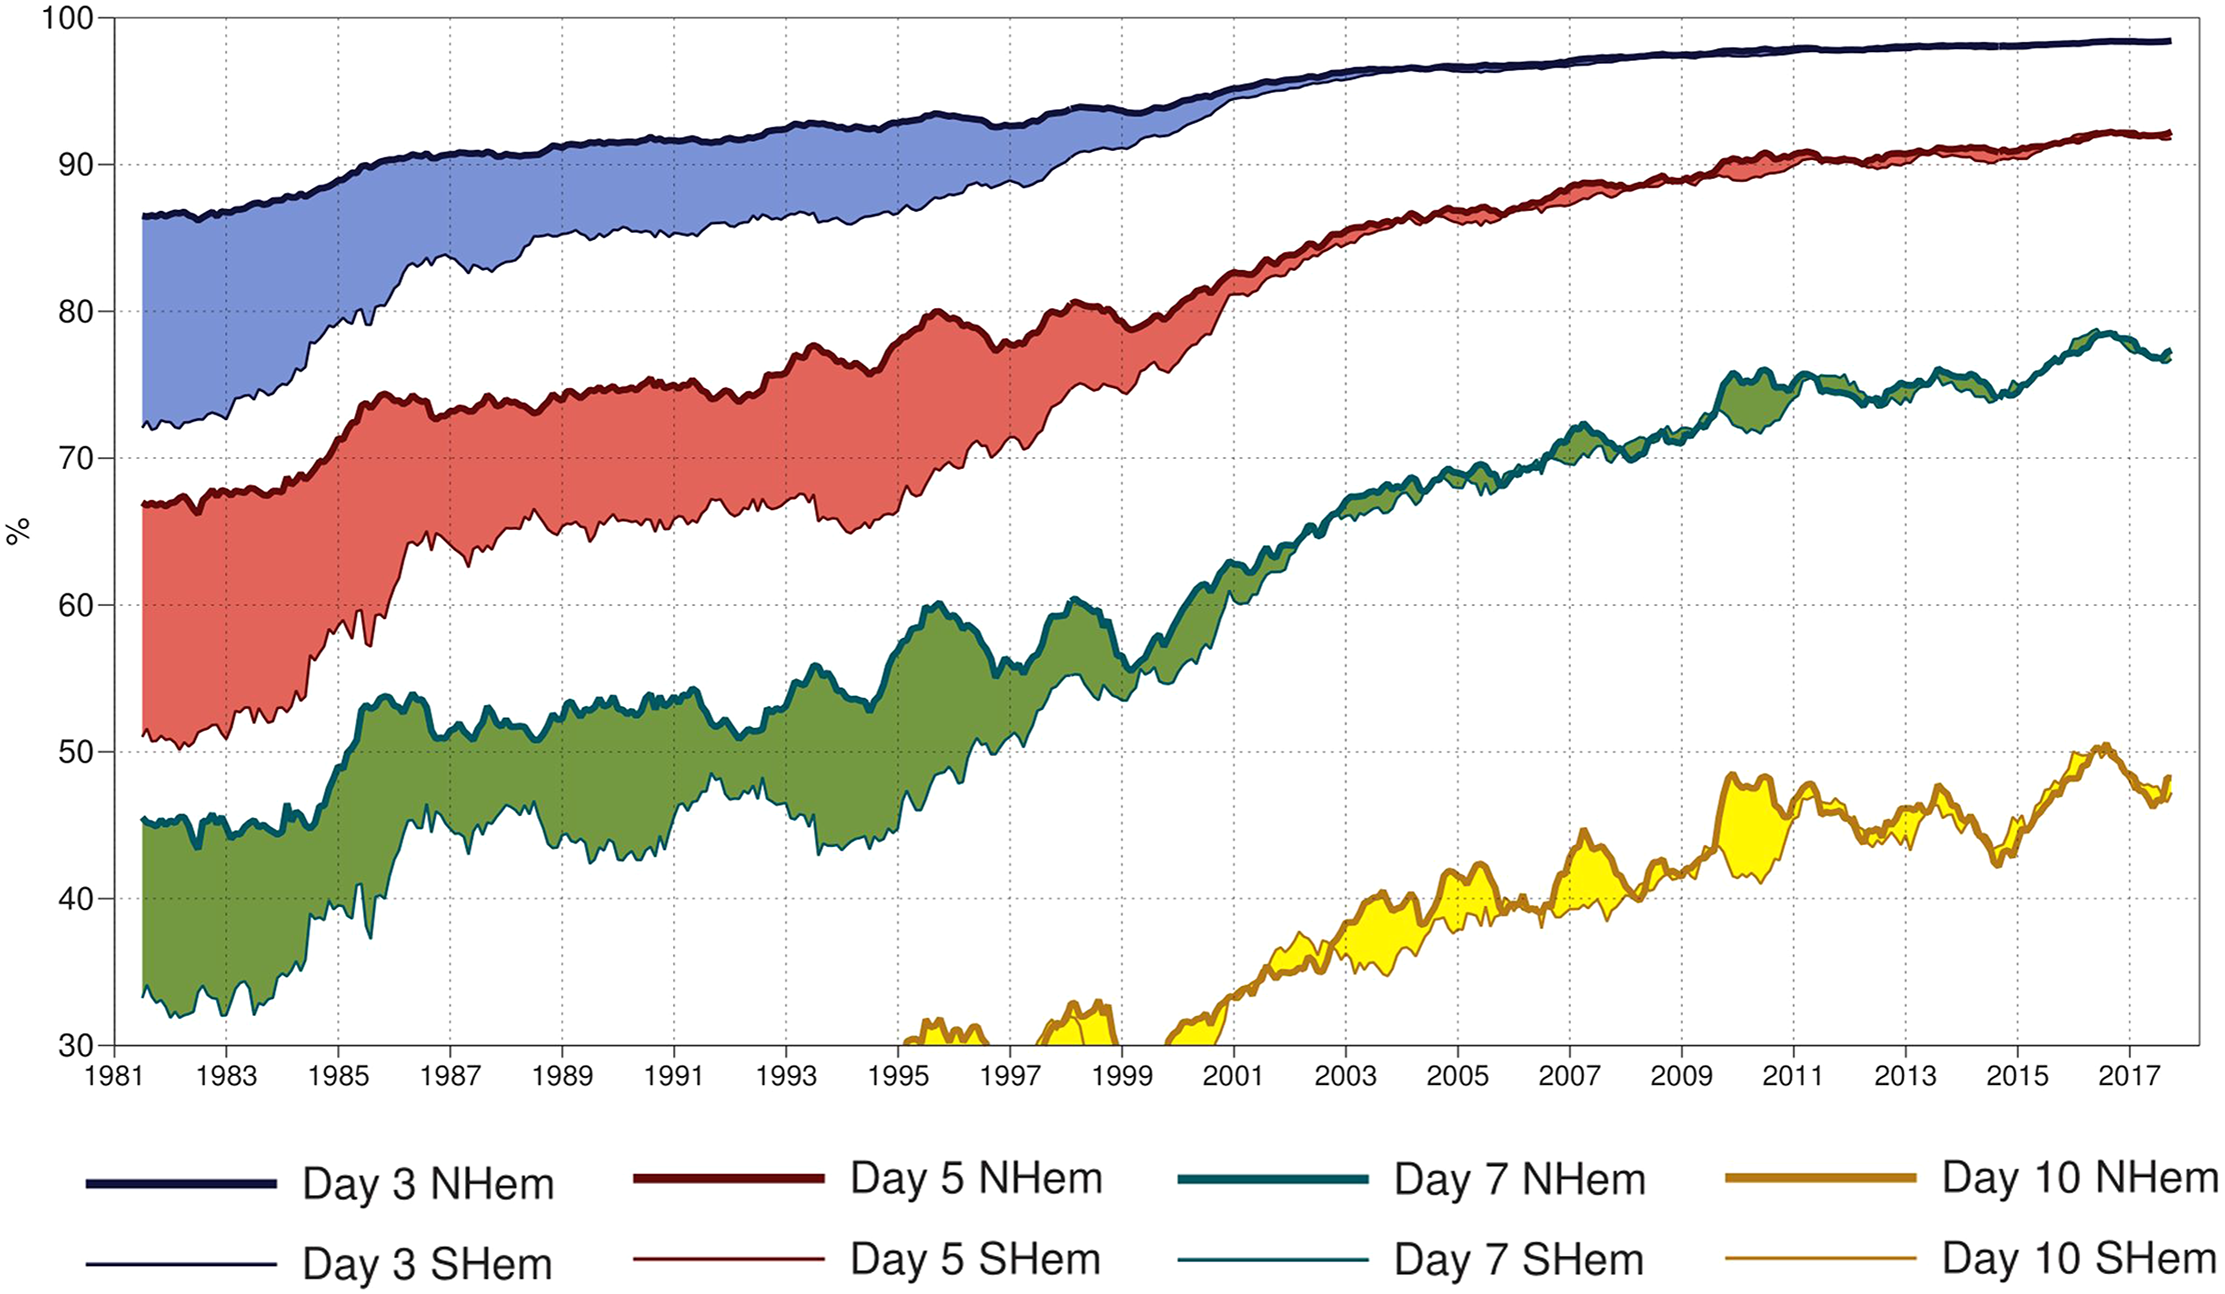
\includegraphics[width=17cm]{figs/zhang.png}
    \caption{From Zhang et al. 2020 \cite{numerical_weather}. The forecasting skill of weather models increasing over time. Colors indicate forecasts for different temporal scales. Original caption: \textit{Annual evolution the ECMWF NWP deterministic control forecast performance in terms of anomaly correlation of 500-hPa-height predictions. Shading indicates the different forecast skill between NH and SH, which has almost disappeared in recent years. This plot is directly adapted from ECMWF official website}}
    \label{fig:num_weather}
\end{figure}

\begin{figure}[h]
    \centering
    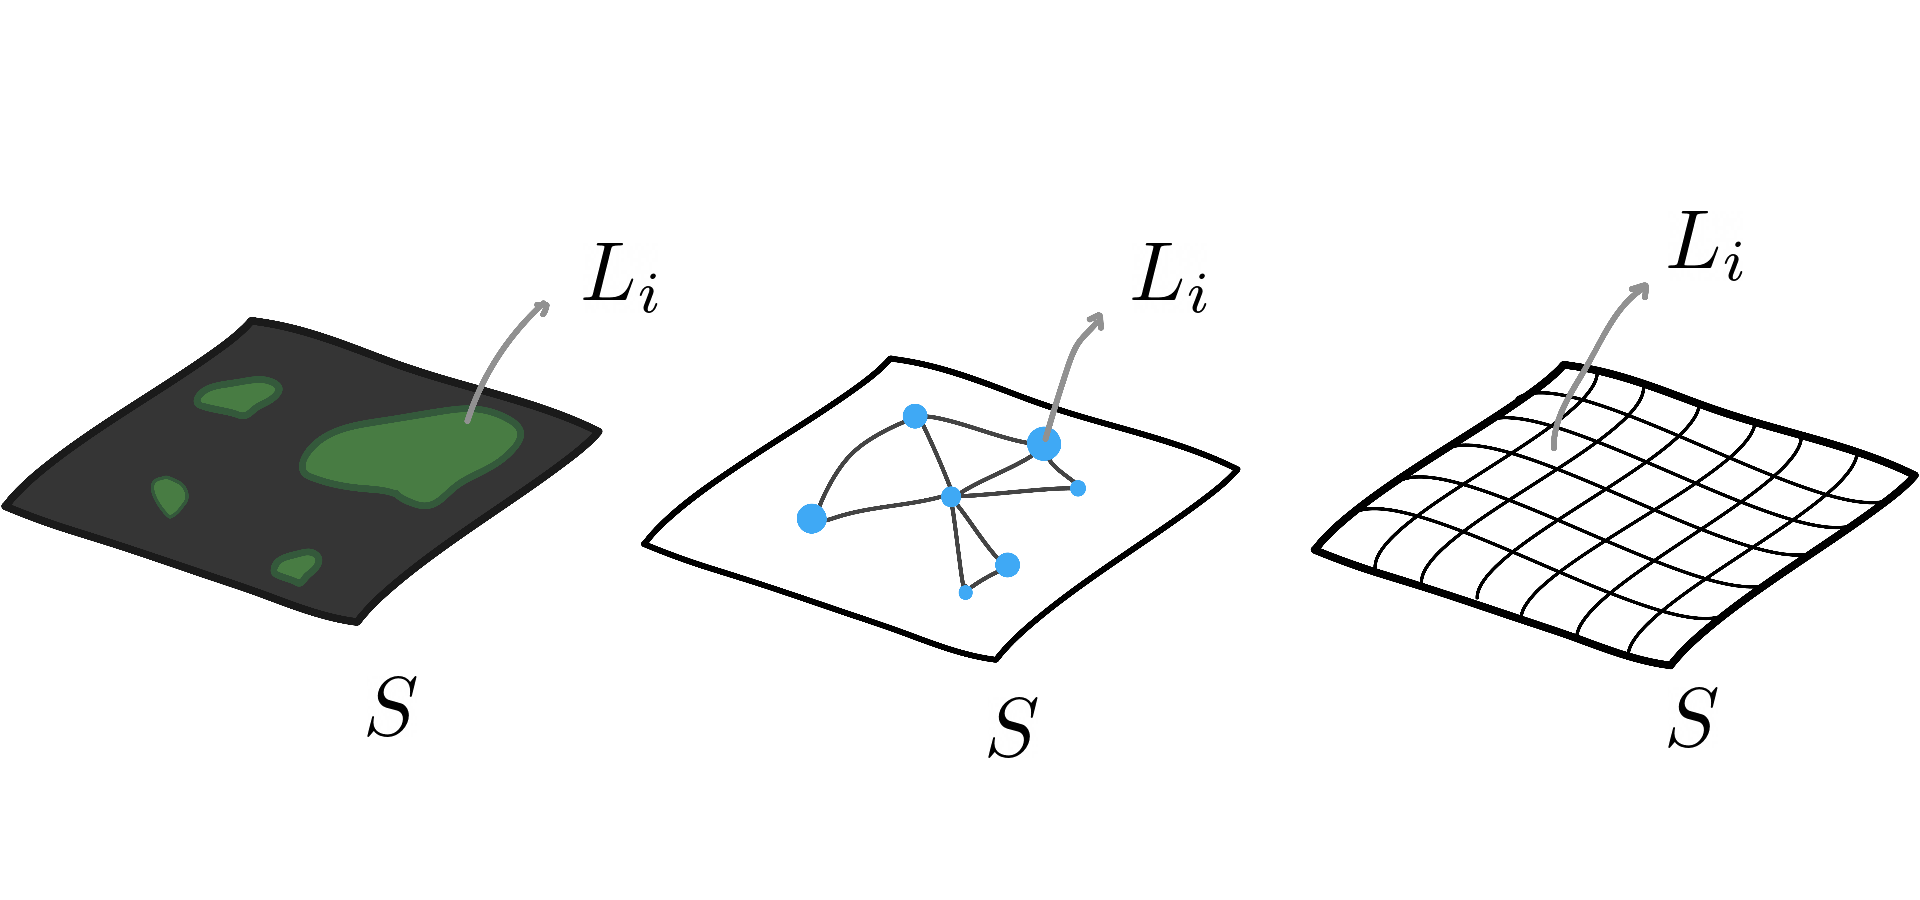
\includegraphics[width=17cm]{figs/different_spatial_models_w_labels.png}
    \caption{Appendix Figure 1: A spatial graph can be used to represent three common landscape representations: patch based, point based, and lattice based. Each landscape consists of a set of nodes $L_i$ in the spatial graph, which are connected by edges, which represent dispersal.  }
    \label{fig:spatial_models}
\end{figure}


\end{document}